\documentclass{article}

\usepackage{graphicx, xcolor}
\usepackage{amsmath, amssymb}
\usepackage[colorlinks=true,allcolors=blue]{hyperref}

\usepackage[margin=1in]{geometry}

\def\hwtitle{Homework 2: Numerical Integration}
\def\hwauthor{Caden Gobat}
\def\hwdate{\today}

\usepackage{fancyhdr}
\lhead{\hwauthor}
\chead{\hwtitle}
\rhead{\hwdate}
\lfoot{\hwauthor}
\cfoot{}
\rfoot{\thepage}
\renewcommand{\footrulewidth}{0.4pt}
\pagestyle{fancy}

\author{\hwauthor}
\title{\hwtitle}
\date{\hwdate}

\begin{document}

\maketitle
\thispagestyle{fancy}

\section{Introduction}

Analytical solutions to differential equations or other applications of integrals are often impractical, overly cumbersome, or outright impossible. Under such conditions, we apply \emph{numerical} integration techniques to arrive at an answer that (we hope) reflects the real solution. There are countless formulae and algorithms for doing this, but a good way to begin conceptualizing it is to consider a basic Riemann sum:
\begin{equation}\label{eq:riemann}
    \int_a^b f(x) dx \approx \sum_{i=1}^n f(x_i) \Delta x
\end{equation}
where $a=x_1$, $b=x_n$, and $\Delta x$ is very small. In the limit as $\Delta x \to 0$, Eq.~\ref{eq:riemann} becomes an equality rather than a mere approximation. For computational purposes however, we have no choice but to use a discrete domain. This assignment will explore the impact of varying levels of discretization, different summation methods, and the accuracy of numerical vs. analytical methods.

\section{Results}

\bigskip
\noindent{\bf Question 1}
\medskip

The plot of $f(x) = \int_0^x e^y dy$ using a left-hand sum is shown in Fig.~\ref{fig:p1_left} at bin widths of 0.02, 0.10, and 0.25, while the result of the analogous midpoint integration is shown in Fig.~\ref{fig:p1_mid}.

\begin{figure}[!h]
    \centering
    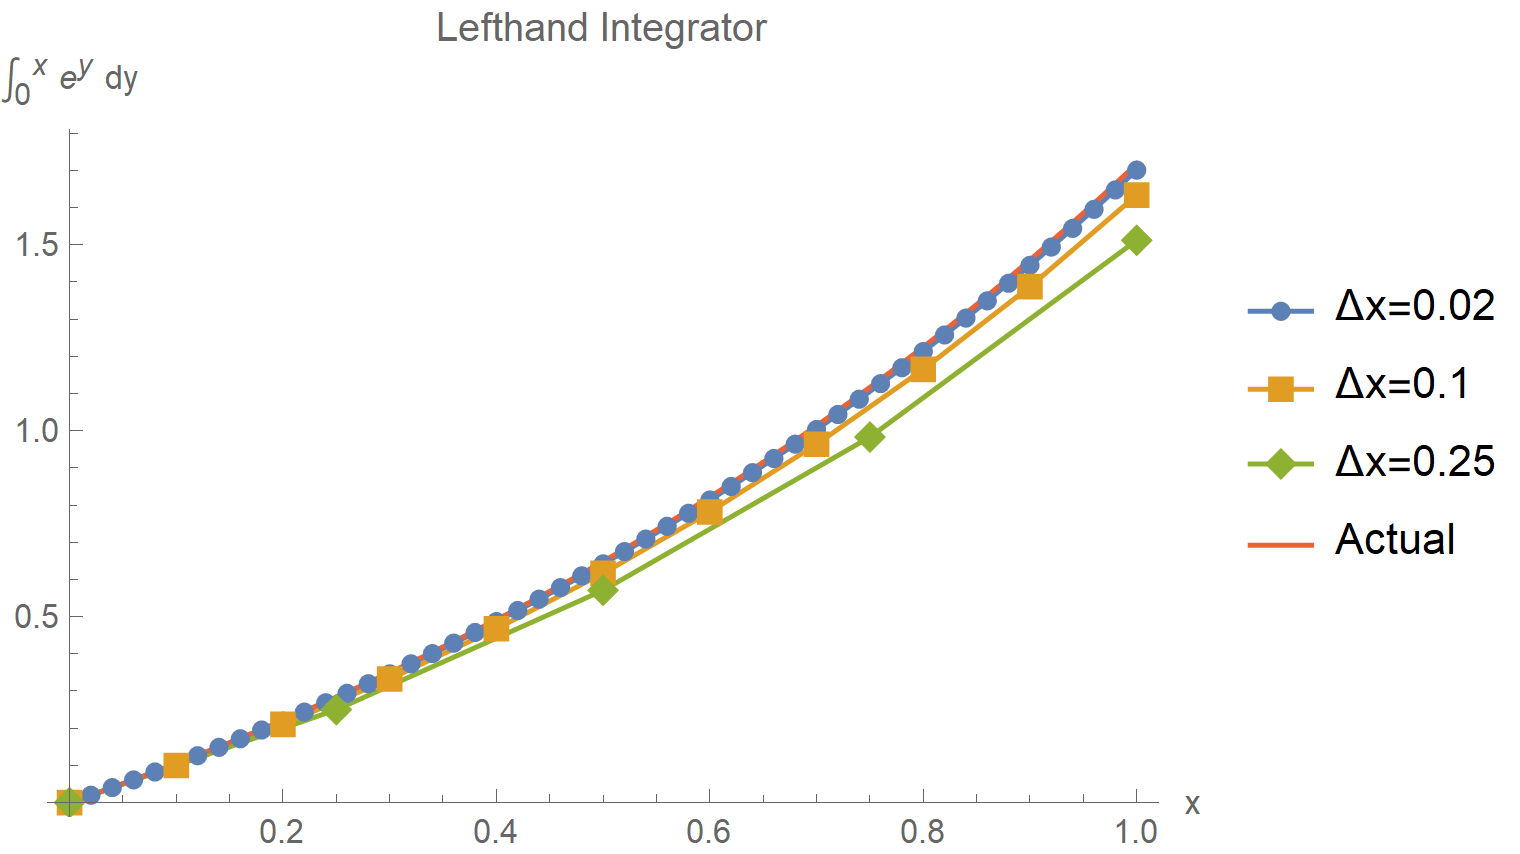
\includegraphics[width=4.75in]{homework2/P1_LH.png}
    \caption{Numerical integration results using the left-hand integrator formula for a variety of bin widths ($\Delta x$). The analytical result is plotted here as the line labeled ``Actual''.}
    \label{fig:p1_left}
\end{figure}

\begin{figure}[!h]
    \centering
    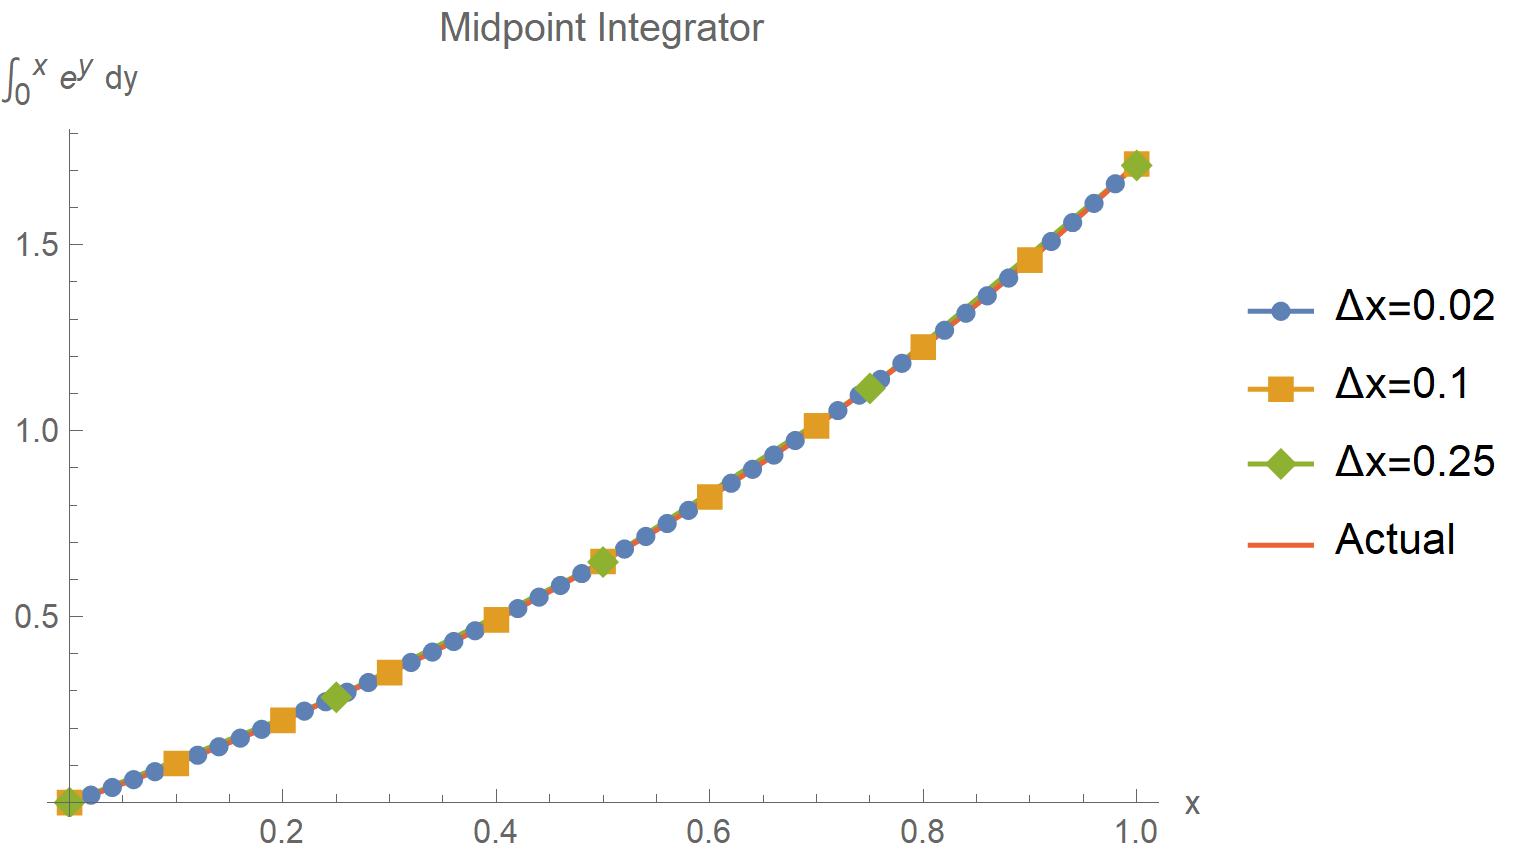
\includegraphics[width=4.75in]{homework2/P1_MP.png}
    \caption{Numerical integration results using the midpoint integrator formula for a variety of bin widths ($\Delta x$). The analytical result is plotted here as the line labeled ``Actual''.}
    \label{fig:p1_mid}
\end{figure}

For both of these, a smaller bin width (and thus more bins in the same domain) leads to higher accuracy when compared to the analytical result.

However, even using fairly large bins, the midpoint method is clearly superior to the left-handed summation. Across the board, the points at each interval of $\Delta x$ are essentially indistinguishable from one another and the analytical solution, meaning that we can afford to use much wider bins when using midpoints rather than left points.

\bigskip
\noindent{\bf Question 2}
\medskip

The integration error for a numerical solution is defined as
\begin{equation}\label{eq:error}
    \epsilon = \frac{|\text{numerical} - \text{analytical}|}{|\text{analytical}|}
\end{equation}

As we saw in the first problem, the error decreases as more bins are used, but more bins also means more computational intensity, so there is a tradeoff. To understand and optimize this, we need to know how the error behaves as a function of bin width or number of bins. Because the integral we are solving is $\int_0^1 e^y dy$, we can determine that
\begin{equation}
    b-a = 1-0 = 1 \implies w = \frac{1}{N}
\end{equation}
where $w$ is the width of one bin and $N$ is the number of bins used.

Plotting $\epsilon$ from Eq.~\ref{eq:error} against this bin width $w$ reveals a distinct relationship (see Fig.~\ref{fig:p2}). By $\log$-scaling both axes, we can see that the relationship becomes linear in logarithmic space. Taking the logarithmic ``slope'':

\begin{equation}\label{eq:logslope}
    \frac{\log(\epsilon_2)-\log(\epsilon_1)}{\log(w_2)-\log(w_1)}
\end{equation}
yields an index of approximately 1. Generally, when a function appears linear in logarithmic space, we say that it is a power law with an index equivalent to the apparent slope of the line. A slope of 1 here means that the original function is of the form $\epsilon \propto w^1$. In other words, it is already linear. Thus we can conclude that the left-handed integration method converges linearly with step size (i.e. step size $h$ has convergence $\mathcal{O}(h^1)$).

\begin{figure}[!h]
    \centering
    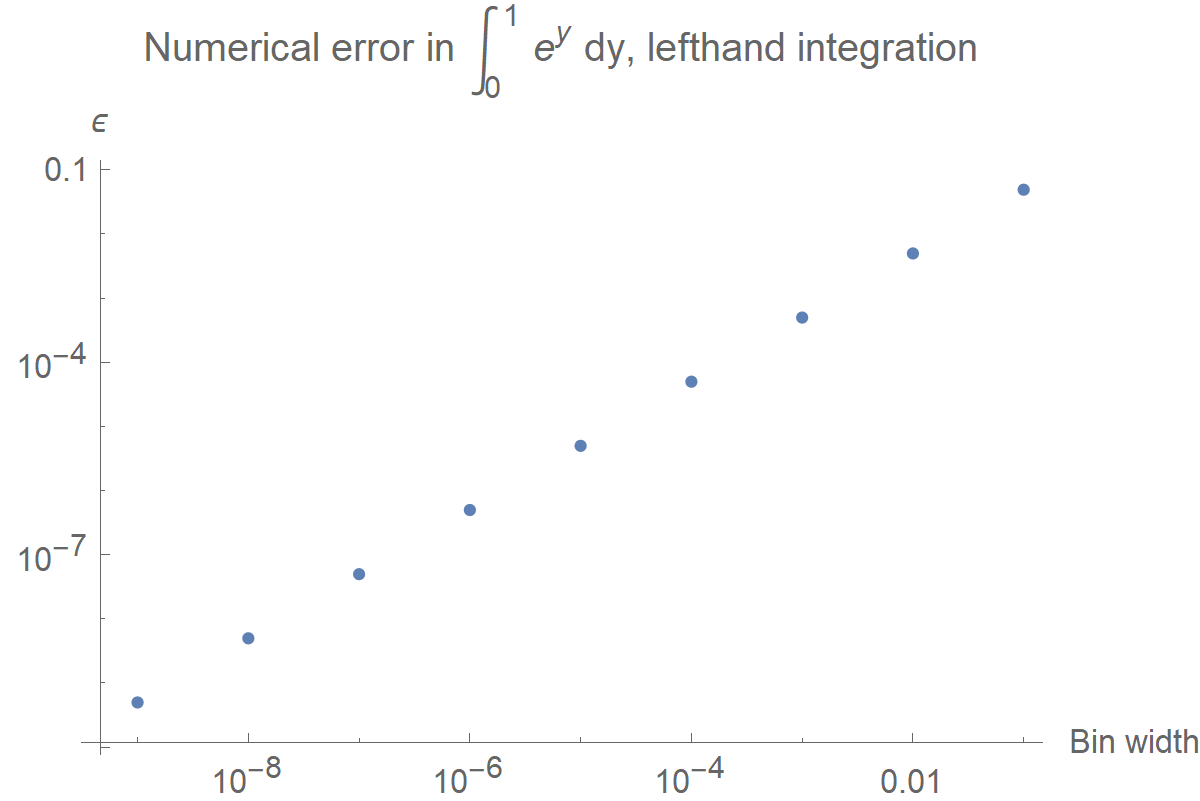
\includegraphics[width=4.75in]{homework2/P2.png}
    \caption{Log-log plot of integration error as a function of bin width. The ``slope'' between the points at $w=10^{-5}$ and $w=10^{-3}$ is $0.999964$.}
    \label{fig:p2}
\end{figure}

\newpage

\bigskip
\noindent{\bf Question 3}
\medskip

Repeating the process of the last problem, we can generate a similar plot of the relationship between bin width and error for the midpoint rule (shown in Fig.~\ref{fig:p3}). Again this plot appears generally linear in logarithmic space, with a slope of approximately 2. This means that the midpoint rule with step size $h$ is convergent on the order $\mathcal{O}(h^2)$, signifying that it is a much more accurate method.

\begin{figure}[!h]
    \centering
    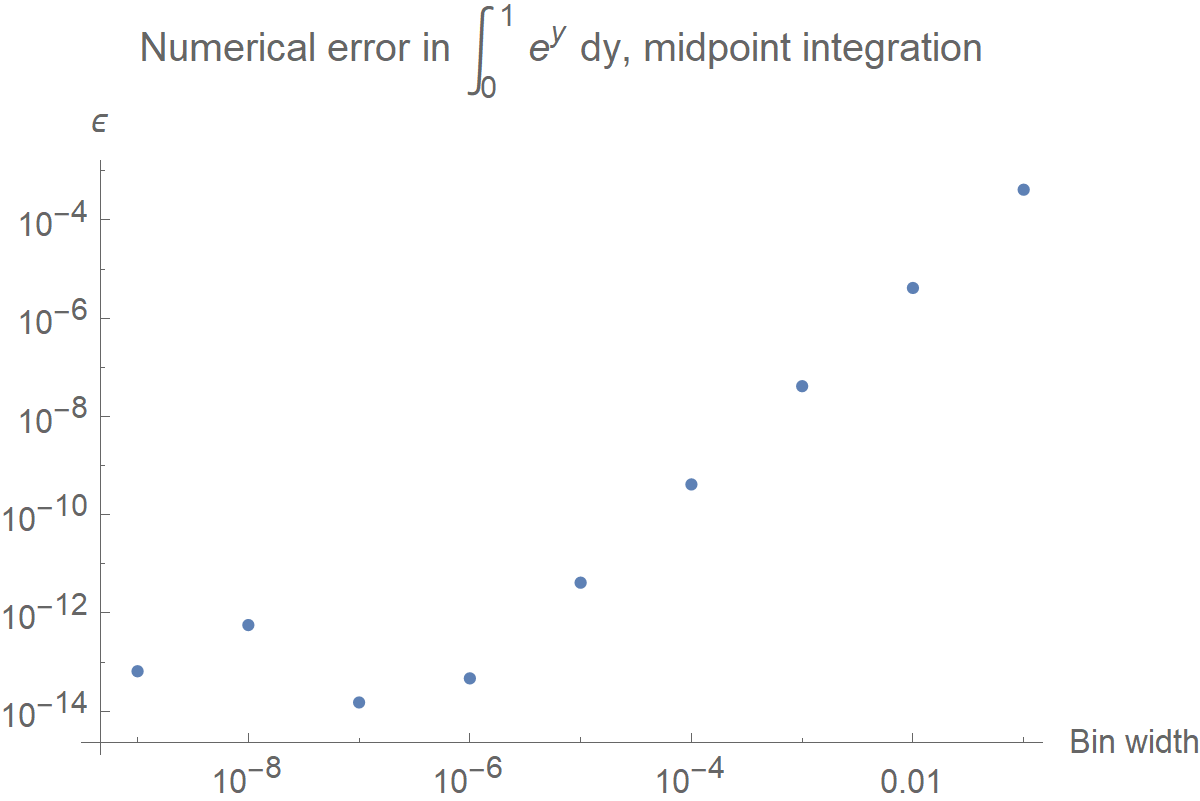
\includegraphics[width=4.75in]{homework2/P3.png}
    \caption{Similar plot concept as in Fig.~\ref{fig:p2}, but this time using the midpoint integration method. The ``slope'' between the points at $w=10^{-5}$ and $w=10^{-3}$ is $1.99991$.}
    \label{fig:p3}
\end{figure}

It is so precise, in fact, that the computer is incapable of fully representing the tiny floating point error at very low bin widths. This phenomenon of floating point representation quirks is what is to blame for the odd behavior of the leftmore three points in Fig.~\ref{fig:p3}. Below a certain point, the computer simply cannot represent the numbers faithfully, so the errors become arbitrarily small. This is why the error graph appears to deviate from the linear trend below $w\simeq10^{-7}$.

\bigskip
\noindent{\bf Question 4}
\medskip

For a small starting angle $\theta_0$, the period of a classical pendulum can be expressed as
\begin{equation} \label{eq:smallangle}
    \tau = 2\pi\sqrt{\frac{L}{g}}
\end{equation}

Of course, we can achieve the same effect computationally using the fact that
\begin{equation}
    \frac{\tau}{2} = \int_{-\theta_0}^{\theta_0}\frac{d\theta}{\omega(\theta)}
\end{equation}
where
\begin{equation}
    \omega(\theta) = \sqrt{\frac{2g}{L}(\cos(\theta)-\cos(\theta_0))}
\end{equation}

This can be done using the same numerical integration techniques we have been using thus far. The point of interest here is how the starting angle $\theta_0$ affects the period.

To keep the numbers simple, I used $g=9.81\text{ m/s}^2$ and $L=9.81$ m, and $N=10^6$ bins. This means we can expect (from Eq.~\ref{eq:smallangle}) the period to be $\tau\approx2\pi$ s. For $\theta_0=15^\circ$, the numerically integrated period is approximately 6.30777 s. This means that over the course of a day, during which it should have completed 13751 cycles, it will only have 13697.4, so if it keeps track of seconds proportionally to elapsed periods, it will be off by around 337 seconds within a day.

Even more critically, a starting angle of $\theta_0=30^\circ$ leads to a period calculation of 6.39 seconds, which means that only 13521 oscillations are made in a day. This will lead to an error of 1445 seconds in one day!

Clearly (and somewhat intuitively), smaller starting angles are more accurate to the analytical determination of the pendulum's period, which uses the small angle approximation that $\theta \simeq \sin(\theta)$, which is only true when $\theta$ is indeed quite small.

\bigskip
\noindent{\bf Bonus Question}
\medskip

Integration error as a function of starting angle is displayed in Fig.~\ref{fig:pendulum} on the next page. The relationship is fairly linear in $\log$-$\log$ space, but gets more accurate even more quickly at smaller angles, when the small angle approximation is truly at its best.

\begin{figure}[!h]
    \centering
    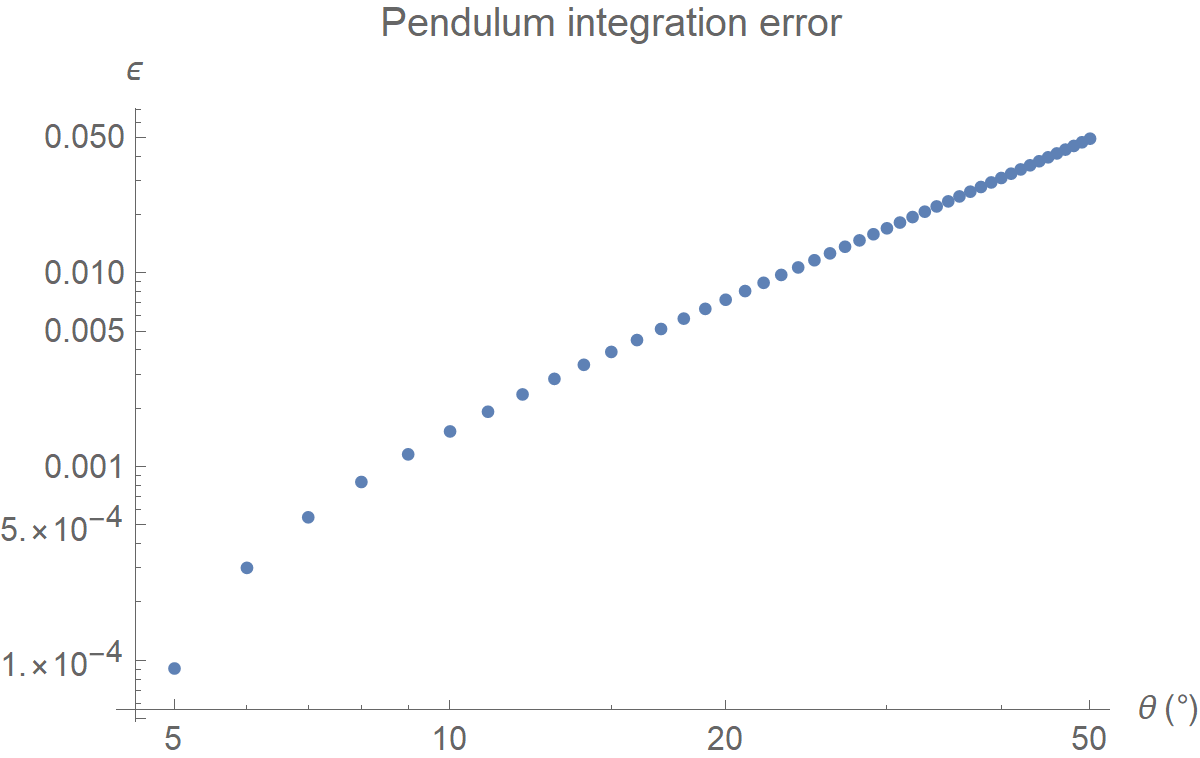
\includegraphics[width=4.75in]{homework2/pendulum.png}
    \caption{Numerical integration error in the pendulum period calculation. The log-slope of the linear part (i.e. between $\theta\approx15^\circ$ and $\theta=50^\circ$) is approximately 2.09.}
    \label{fig:pendulum}
\end{figure}

For the part that is clearly linear, the logarithmic slope is just under 2.1. As before, this implies that for a $\sin$-based function, midpoint integration has convergence $\mathcal{O}(\theta_0^{2.1})$. However, this is not exactly analogous to previous convergence orders, as this power law is over a domain of initial condition possibilities rather than number of bins or bin width. This means that the graph shows less about return on increasing computational complexity and more about the rate at which using a small angle approximation becomes problematic.

\newpage

\section{Conclusions}

These exercises demonstrated both the power and the limitations of numerical integration techniques. A multitude of factors go into determining the accuracy with which a numerical integrator can be used, such as algorithm, step size, domain range, type of integrand, and even initial (starting) conditions.

We saw that for an exponential, the order of convergence for midpoint summation goes as $h^2$, whereas that of lefthand summation is linear in $h$. The most challenging piece of this assignment for me personally was understanding this kind of pseudo big-$\mathcal{O}$ notation to talk about the rates at which different algorithms converge to the analytical solution.

In all, this assignment went well and I came away with a better understanding of how to implement numerical methods in C.

\end{document}
